\documentclass[pscyr]{hedlab}
\usepackage[russian]{babel}
\usepackage{graphicx}
\graphicspath{{images/}}
\usepackage{listings}

\lstset{
  basicstyle=\footnotesize,
  inputencoding=koi8-r,
  extendedchars=True,
  language=[Sharp]C,
  numbers=left,
  numberstyle=\footnotesize,
  breakatwhitespace=\false,
  breaklines=True,
  tabsize=2,
  keepspaces=true,
}

\labname{Публикация данных в веб\\Часть 2}
\labnum{4}
\student{Чечеткин И. А., САПР-1.1п}
\labdate{}

\begin{document}
    \makeheader
    \emph{Цель:} получить практические навыки добавления, редактирования и удаления данных из 
    веб-приложения с использованием компонент SQLDataSource и GridView.\\
    \emph{Задачи:} 
    \begin{enumerate}
        \item Создать базу данных из связанных таблиц произвольной предметной области.
        \item Осуществить подключение к базе данных с использованием компонент SQLDataSource.
        \item Отобразить данные с помощью объекта класса GridView.
        \item Реализовать метод добавления данных в таблицу базы данных.
        \item Реализовать метод корректировки данных в таблице базы данных непосредственно в 
            объекте класса GridView.
        \item Реализовать метод удаления данных из таблицы базы данных.
    \end{enumerate}
    Реализация работы с таблицой БД:
    \lstinputlisting{code/orderdetail.aspx.cs}
    \pagebreak
    Страница с элементами GridView и SqlDataSource:
    \lstinputlisting[language=HTML]{code/orderdetail.aspx}

    \pagebreak
    Скриншоты с Web-страниц с БД:
    \begin{figure}[h!]
      \center
      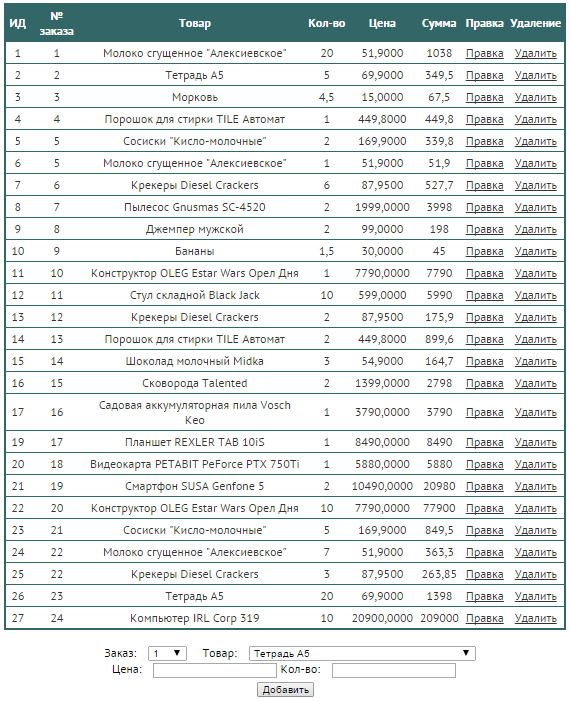
\includegraphics[width=.47\textwidth]{01} \hspace{1em}
      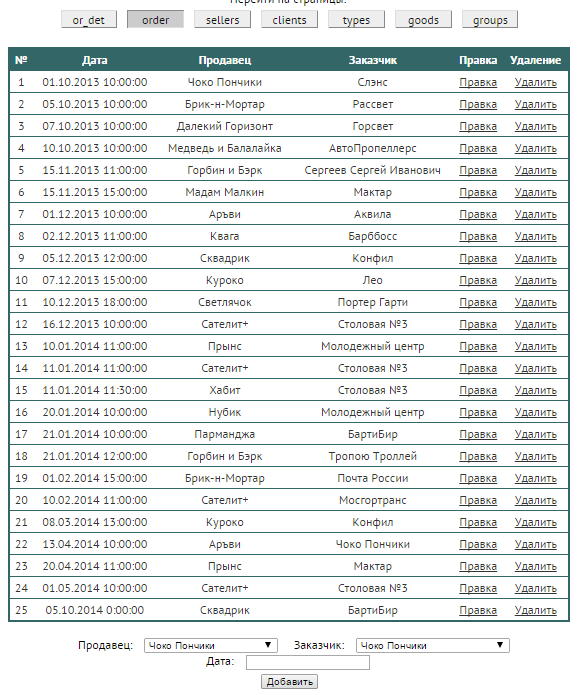
\includegraphics[width=.47\textwidth]{02} \\
      \parbox{.47\textwidth}{\center Страница OrderDetail} \hspace{1em}
      \parbox{.47\textwidth}{\center Страница Order} \\
      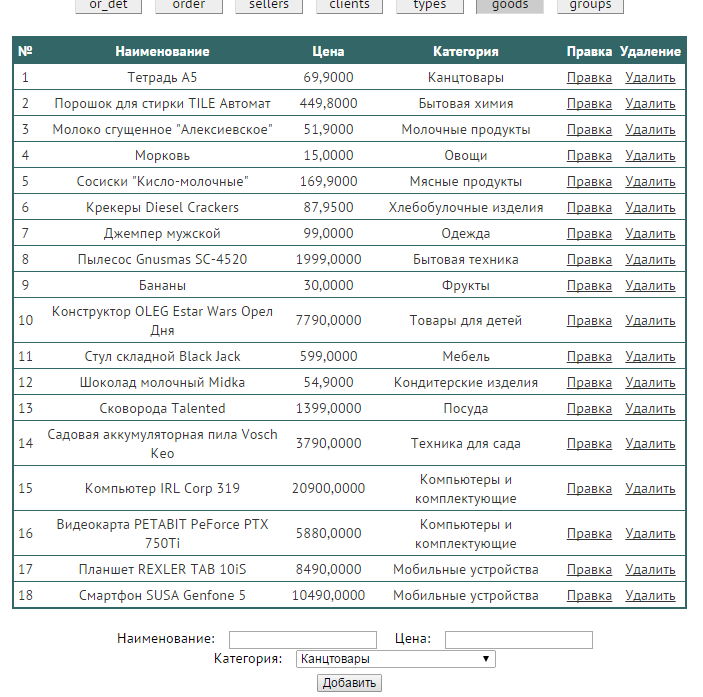
\includegraphics[width=.47\textwidth]{03} \hspace{1em}
      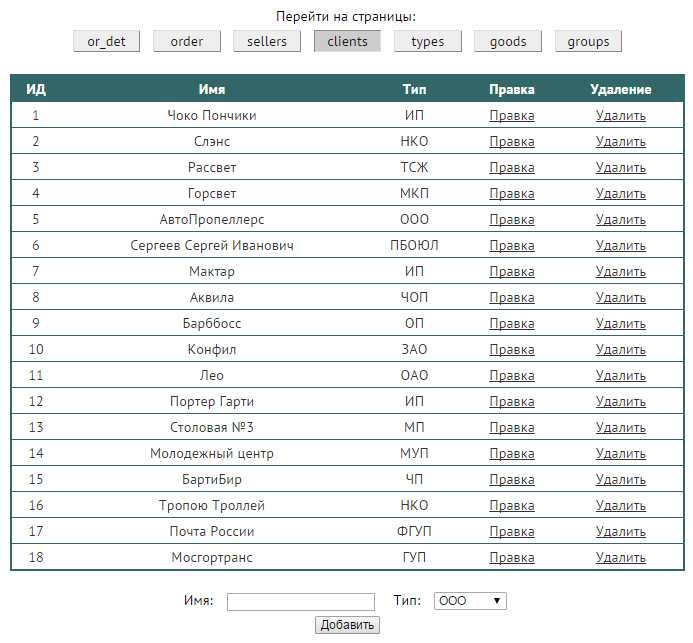
\includegraphics[width=.47\textwidth]{04}
      \parbox{.47\textwidth}{\center Страница Goods} \hspace{1em}
      \parbox{.47\textwidth}{\center Страница Clients} \\
    \end{figure}
    \pagebreak
    \begin{figure}[h!]
        \center
        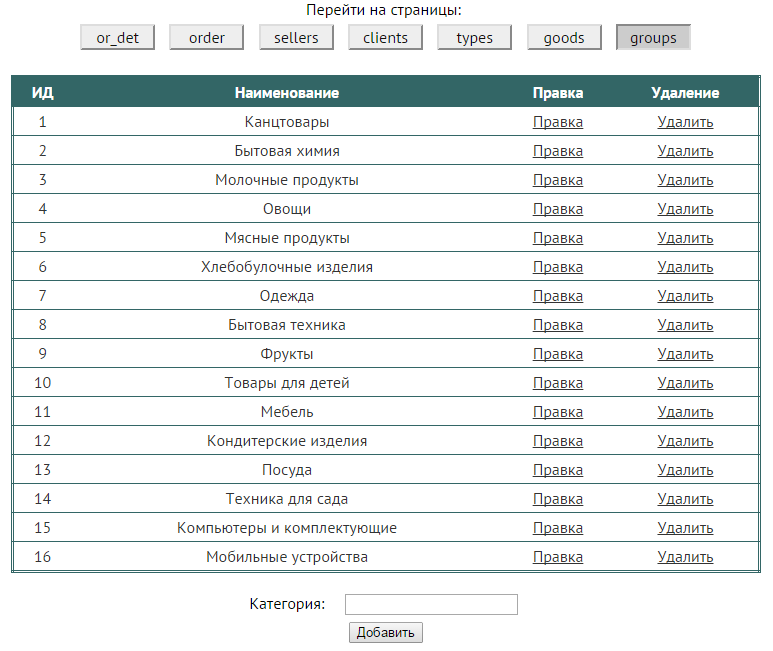
\includegraphics[width=.47\textwidth]{05} \hspace{1em}
        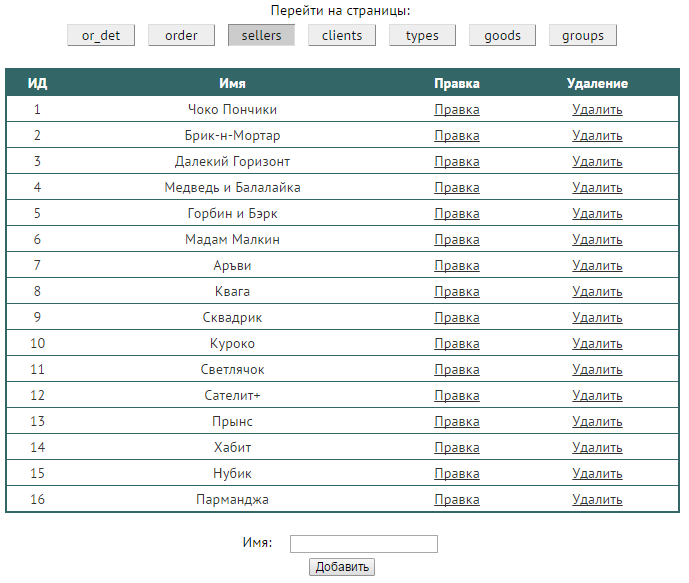
\includegraphics[width=.47\textwidth]{06} \\
        \parbox{.47\textwidth}{\center Страница Groups} \hspace{1em}
        \parbox{.47\textwidth}{\center Страница Sellers} \\
        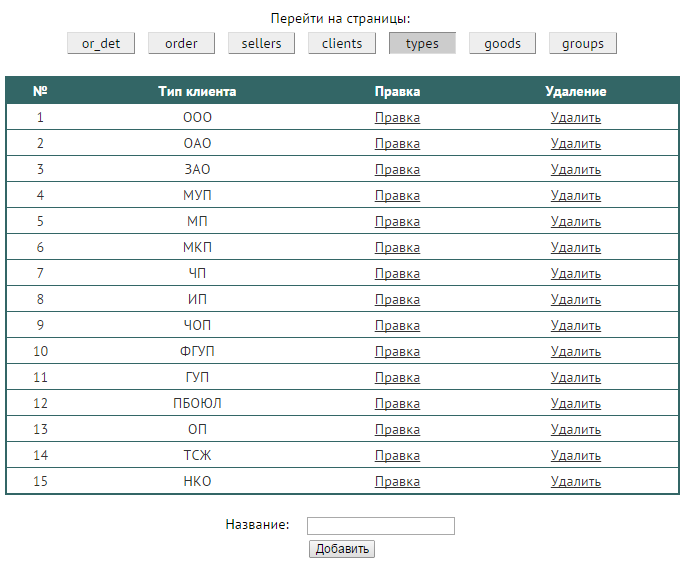
\includegraphics[width=.47\textwidth]{07} \\
        \parbox{.47\textwidth}{\center Страница Types}
    \end{figure}

    \emph{Вывод:} в результате проделанной работы
    \begin{enumerate}
        \item Создал базу данных из связанных таблиц произвольной предметной области.
        \item Осуществили подключение к базе данных с использованием компонент SQLDataSource.
        \item Отобразили данные с помощью объекта класса GridView.
        \item Реализовали метод добавления данных в таблицу базы данных.
        \item Реализовали метод корректировки данных в таблице базы данных непосредственно в объекте 
        класса GridView.
        \item Реализовали метод удаления данных из таблицы базы данных.
    \end{enumerate}

\end{document}